Tenants have exit options, too.  The default rule is that a tenant's interest in
a term of years lease or periodic tenancy is also freely transferable.  (Note,
however, that a tenant cannot transfer a tenancy at will to another party.) 
The law recognizes two types of transfer: the \term{assignment} and
the \term{sublease}.  The vast majority of jurisdictions use an objective
test to distinguish the two.  In an assignment, the original tenant transfers
all of the remaining interest under the lease to a new tenant.  In a sublease,
on the other hand, the original tenant transfers less than all of her remaining
rights in the unexpired period---the original tenant either gets the unit back
at the end of the sublease or reserves a right to cut the sublease short.  

An example should illuminate the concepts.  Imagine that the Witch leases her
Gingerbread Cottage to Hansel for a period of one year---January 1 to December
31---in exchange for \$100 a month.  Four months into the lease, Hansel then
transfers all of his remaining interest in the property to Gretel so that she
now has exclusive possessory rights until the end of the term.  This transfer,
shown in the left part of Figure~\ref{f:lease-assignment},
is an assignment because Hansel has no further rights in the property.  If
Hansel had retained for himself the final two months of the lease or if he'd
rented the cottage to Gretel for only the summer months, we would then
categorize the agreement as a sublease.

\usetikzlibrary{positioning,arrows.meta,quotes}
\begin{figure}
\begin{center}
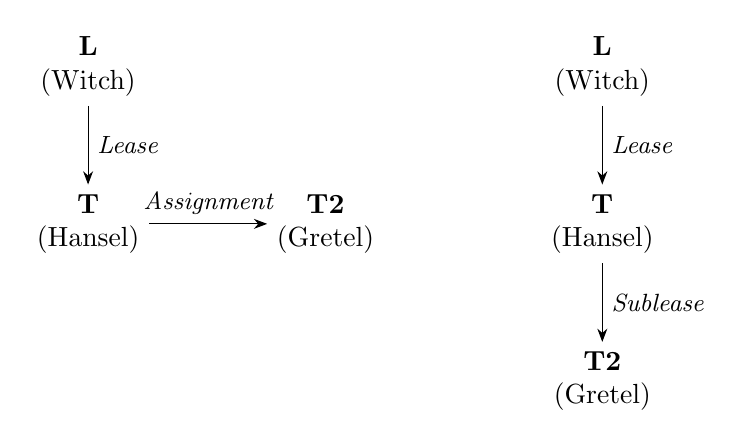
\begin{tikzpicture}
\draw[
    every node/.style={align=center},>=Stealth,->,
    every edge quotes/.style={auto, node font=\itshape\small},
]
node (l) {\textbf{L} \\ (Witch)}
node[below=of l] (t) {\textbf{T} \\ (Hansel)}
node[right=1.5cm of t] (t2) {\textbf{T2} \\ (Gretel)}
(l) edge["Lease"] (t)
(t) edge["Assignment"] (t2)

node[right=2cm of t2] (st) {\textbf{T} \\ (Hansel)}
node[above=of st] (sl) {\textbf{L} \\ (Witch)}
node[below=of st] (st2) {\textbf{T2} \\ (Gretel)}
(sl) edge["Lease"] (st)
(st) edge["Sublease"] (st2)
;
\end{tikzpicture}
\end{center}
\caption{Diagram of an assignment and sublease. Downward arrows will always
represent (sub)leases, while rightward arrows will represent assignments.}
\label{f:lease-assignment}
\end{figure}

A minority of jurisdictions takes a less formalistic approach to the
assignment/sublease division.  In these states, the subjective intent of the
parties, rather than the structure of the transaction, controls.  Arkansas, for
example, allows parties to designate their leases as subleases or assignment
(and receive all the attendant rights and obligations under the chosen
category) regardless of whether the new tenant takes the unit for the entire
remaining term.  

The distinction between subleases and assignments has a few significant legal
consequences.  Primarily, it affects who can benefit from the promises in the
original lease and who is on the hook for the obligations.  Think again about
the Hansel and Gretel example described above.  If Gretel, who took over the
lease, stops making rent payments, whom can the landlord sue?  The original
tenant, Hansel?  Gretel?  Both?  What if the original one-year lease contained
a provision allowing the tenant to renew for a second year with the same terms?
 Can Gretel take advantage of that clause?  

To enforce any promise, the law requires a certain type of legal relationship
between the parties, known as \textit{privity}.  Donald Trump, for example,
cannot successfully sue you if one of his Trump Tower tenants suddenly fails to
pay rent---there's simply no connection between Trump and you.  Trump could
only sue you if a privity relationship exists: either \term{privity of
contract} or \term{privity of estate}.  Privity of contract is easy enough to
understand.  Parties are in privity of contract if they have entered into a
valid contract with each other.  In our example, the Witch and Hansel are in
privity of contract because they signed the original lease agreement.  The
Witch gave Hansel the right to exclusive possession for one year and Hansel
promised to pay rent every month.  As a result of this legal relationship, the
Witch has the option to sue Hansel if she doesn't receive rent.  That remains
true even if Hansel transfers his lease to someone else.  That bears repeating:
the original tenant's promise to pay the landlord stands until the original
lease expires (or until the landlord releases the tenant from this obligation).
 
When Hansel and the Witch first sign the lease, they also stand in privity of
estate with each other.  This concept is yet another holdover from feudal
times.  Privity of estate makes concrete the medieval belief that an individual
takes on a series of rights and obligations when they occupy land owned by
another.\footnote{The medieval mind thought of rent as something that came
from the land itself: the tenant paid the land-\textit{lord} out of the fruits
of the land, sometimes metaphorically but sometimes literally, with crops
harvested from the land being leased.}  For our purposes, privity of estate
arises when two parties have successive ownership claims in the same property.
Hansel and the Witch have privity of estate because once Hansel's possessory
interest concludes, his property rights flow immediately back to the Witch. 
Despite its archaic origin, the idea remains important in modern property law
because individuals in privity of estate can sue each other directly for (some)
violations of a rental agreement.\having{intro-covenants}{}{\footnote{We'll
learn more about which promises ``run with the land'' in \mref{intro-covenants}.
For now, it's enough to know that transferees can only enforce
promises that concern the property or land.}}{The property law concept of
``covenants,'' not covered in this book, deals with which promises ``run with
the land.'' For now, it's enough to know that transferees can only enforce
promises that concern the property or land.}

Consider, again, what happens when Hansel transfers his rights in the
gingerbread cottage to Gretel.  Can the Witch successfully haul Gretel into
court if she stops making payments?  It should be obvious that Gretel has not
made any direct agreement with the Witch (or made any promise to benefit her)
so they are not in privity of contract.  But what about privity of estate? 
This is where the distinction between assignments and subleases matters.  If
Hansel assigns his interest to Gretel, then Gretel and the Witch would be in
privity of estate (and the Witch could sue Gretel for the missing rent).  We
know they have privity of estate because when Gretel's rights end under the
assignment, the Witch would immediately be entitled to exclusive possession of
the cottage---they have successive interests in the same piece of real estate. 
Conversely, if Hansel subleases his apartment to Gretel for the summer, a
privity relationship would not arise between Gretel and the Witch.  Instead,
Gretel would have privity of estate with Hansel because at the conclusion of
Gretel's interest, Hansel would have the right to exclusive possession.  Thus,
under the sublease, the Witch could not sue Gretel for rent.

Figuring out which parties stand in privity of estate can initially cause a lot
of confusion.  However, asking two quick questions can help define these
relationships.  The first step is to ask, ``Have any tenants made an assignment
of their rights?''  If a tenant has assigned their rights they have no chance
of possessing the property again and, thus, cannot stand in privity of estate
with anyone (although they may still be in privity of contract with various
parties).  For all the remaining tenants ask, ``Who receives the property when
this tenant's possessory rights finally end?''  Remember, parties with
successive interests have privity of estate. 

\begin{figure}
\begin{center}
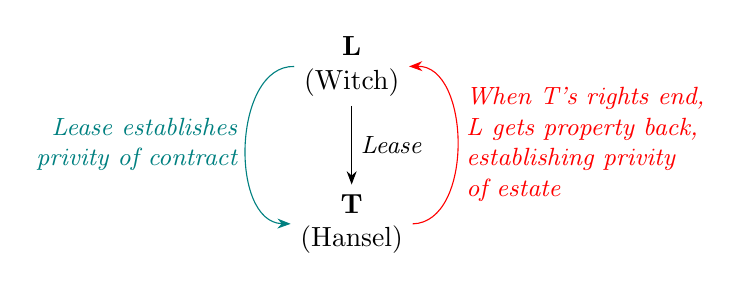
\begin{tikzpicture}
\draw[
    every node/.style={align=center},>=Stealth,->,
    every edge quotes/.style={auto, node font=\itshape\small},
]
node (l) {\textbf{L} \\ (Witch)}
node[below=of l] (t) {\textbf{T} \\ (Hansel)}
(l) edge["Lease"] (t)
    edge[bend right=90, "Lease establishes\\privity of contract"
        {left,align=right}, teal] (t)
(t) edge[bend right=90, "{When T's rights end,\\L gets property
        back,\\establishing privity\\of estate}" {right,align=left}, red] (l)
;
\end{tikzpicture}
\end{center}
\caption{Privity of contract and estate for leases.}
\label{f:lease-privity}
\end{figure}

Although it may be redundant, a few diagrams may help clarify these
relationships.  Assume that L leases an apartment to T.  Whenever a landlord
initially leases to a tenant the two parties are in both privity of contract
and privity of estate, as shown in Figure~\ref{f:lease-privity}.

%\heregraphic{leases-07}
L and T are in privity of contract because they agreed on a lease contract. To
figure out the privity of estate relationships, we first ask if anyone has
assigned their interest.  The answer here is ``no.''  For all remaining
tenants, we inquire ``who gets control over the property when this tenant's
possessory rights end?''  In this hypothetical, who gets the leased premise
when T's term concludes?  The answer, of course, is the landlord. T and L are
in privity of estate because the landlord gets the property back from the
tenant at the end of the lease.  

\begin{figure}
\begin{center}
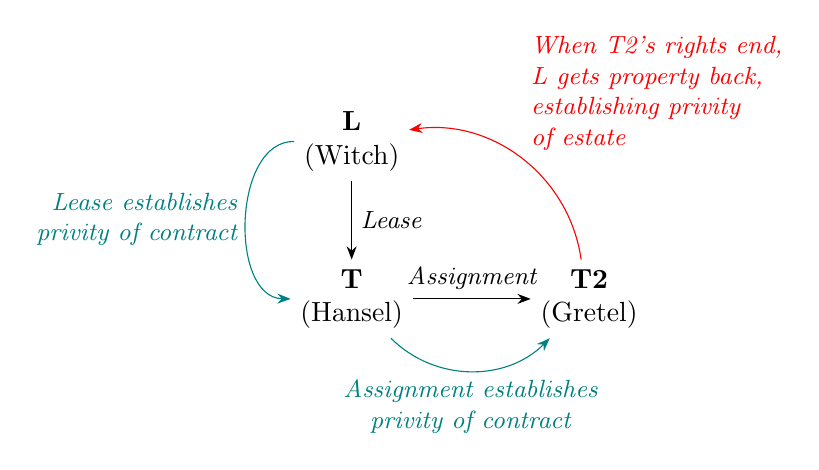
\begin{tikzpicture}
\draw[
    every node/.style={align=center},>=Stealth,->,
    every edge quotes/.style={auto, node font=\itshape\small},
]
node (l) {\textbf{L} \\ (Witch)}
node[below=of l] (t) {\textbf{T} \\ (Hansel)}
node[right=1.5cm of t] (t2) {\textbf{T2} \\ (Gretel)}
(l) edge["Lease"] (t)
    edge[bend right=90, "Lease establishes\\privity of contract"
        {left,align=right}, teal] (t)
(t) edge["Assignment"] (t2)
    edge[bend right=45, "Assignment establishes\\privity of contract" below,
        teal] (t2)
(t2) edge[bend right=45, "{When T2's rights end,\\L gets property
        back,\\establishing privity\\of estate}" {above right,align=left}, red]
        (l)
;
\end{tikzpicture}
\end{center}
\caption{Privity of contract and estate following an assignment.}
\label{f:lease-privity-assignment}
\end{figure}

The relationships change if T assigns his rights to a new party, T2.  The
diagram of an assignment is in Figure~\ref{f:lease-privity-assignment}.



%\heregraphic{leases-08}
The contractual relationships are easy enough to map.  As discussed earlier,
when T assigns his interest, he remains in privity of contract with L---they
signed a rental agreement that has not expired.  T and T2 are also in privity
of contract as a result of the assignment contract.  But what about privity of
estate?  L and T are no longer in privity of estate because T has relinquished
all of his property interests.  Remember that parties who assign their rights
stand in privity of estate with no one.  For all other tenants we ask, ``Who
receives the property when this tenant's possessory rights finally end?'' When
T2's possessory rights conclude, who takes control of the property? The answer
is the landlord.  L and T2 now have a privity of estate relationship.  

\begin{figure}
\begin{center}
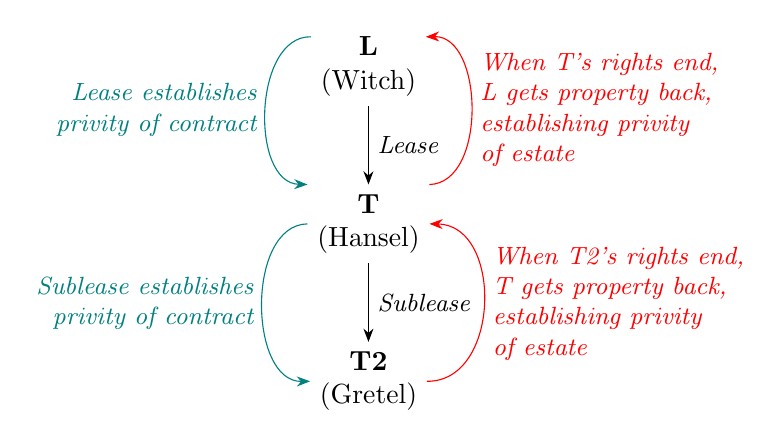
\begin{tikzpicture}
\draw[
    every node/.style={align=center},>=Stealth,->,
    every edge quotes/.style={auto, node font=\itshape\small},
]
node (l) {\textbf{L} \\ (Witch)}
node[below=of l] (t) {\textbf{T} \\ (Hansel)}
node[below=of t] (t2) {\textbf{T2} \\ (Gretel)}
(l) edge["Lease"] (t)
    edge[bend right=90, "Lease establishes\\privity of contract"
        {left,align=right}, teal] (t.north west)
(t) edge["Sublease"] (t2)
    edge[bend right=90, "Sublease establishes\\privity of contract"
        {left,align=right}, teal] (t2)
(t2) edge[bend right=90, looseness=1.2, "{When T2's rights end,\\T gets property
        back,\\establishing privity\\of estate}" {right,align=left}, red]
        (t)
;
\draw[red,-Stealth,
    every edge quotes/.style={auto, node font=\itshape\small},
]
(t.north east) to[bend right=90, "{When T's rights end,\\L gets property
        back,\\establishing privity\\of estate}" {right,align=left}, red] (l)
;
\end{tikzpicture}
\end{center}
\caption{Privity of contract and estate following a sublease.}
\label{f:lease-sublease-privity}
\end{figure}

How do things change with a sublease? In Figure~\ref{f:lease-sublease-privity},
T remains in privity of contract with L for the duration of the
original lease.  In this example, there are no assignments, so we begin by
asking which parties have successive property interests.  When the possessory
rights of T2 end, T will then have control over the property.  Thus T2 and T
have a privity of estate relationship.  Then, when T's rights over the property
conclude, the possessory rights will flow back to the landlord, meaning that T
and L also have privity of estate.  

Before moving on, one final wrinkle merits attention.  As discussed earlier,
when the original tenant subleases or assigns his leasehold, the default rule
is that the landlord and the new tenant are not in privity of contract.  It is
possible, however, to create a privity of contract relationship between the L
and T2.  Most often this is accomplished by including a clause in the takeover
agreement between the original tenant and the new tenant that reads, ``New
Tenant assumes the obligation to perform all of the original tenant's duties
under the original lease.''  If the new tenant takes on this responsibility,
the landlord becomes a third-party beneficiary to the agreement and comes into
privity of contract with the new tenant.  

